\documentclass{article}

% Recommended, but optional, packages for figures and better typesetting:
\usepackage{microtype}
\usepackage{graphicx}
\usepackage{booktabs} % for professional tables 

% hyperref makes hyperlinks in the resulting PDF.
% If your build breaks (sometimes temporarily if a hyperlink spans a page)
% please comment out the following usepackage line and replace
% \usepackage{icml2020} with \usepackage[nohyperref]{icml2020}.
\usepackage{hyperref}

% Attempt to make hyperref and algorithmic work together better:
\newcommand{\theHalgorithm}{\arabic{algorithm}}

% Use the following line for the initial blind version submitted for review:
%\usepackage{icml2020}

% If accepted, instead use the following line for the camera-ready submission:
\usepackage[accepted]{icml2020}

% The \icmltitle you define below is probably too long as a header.
% Therefore, a short form for the running title is supplied here:
\icmltitlerunning{Integrating Logical Rules Into Neural Multi-Hop Reasoning for Drug Repurposing}


\usepackage{graphicx}
\usepackage{subcaption}
\captionsetup{compatibility=false, labelsep=period, labelfont=bf}
\usepackage[export]{adjustbox}
\usepackage{amsmath, amssymb}
\usepackage{dsfont}
\DeclareMathOperator*{\argmax}{arg\,max}
   
\renewcommand{\thefootnote}{3}

\begin{document}

\twocolumn[
\icmltitle{Integrating Logical Rules Into Neural Multi-Hop Reasoning\\ for Drug Repurposing}

% It is OKAY to include author information, even for blind
% submissions: the style file will automatically remove it for you
% unless you've provided the [accepted] option to the icml2020
% package.

% List of affiliations: The first argument should be a (short)
% identifier you will use later to specify author affiliations
% Academic affiliations should list Department, University, City, Region, Country
% Industry affiliations should list Company, City, Region, Country

% You can specify symbols, otherwise they are numbered in order.
% Ideally, you should not use this facility. Affiliations will be numbered
% in order of appearance and this is the preferred way.
\icmlsetsymbol{equal}{*}

\begin{icmlauthorlist}
\icmlauthor{Yushan Liu}{equal,siemens,lmu}
\icmlauthor{Marcel Hildebrandt}{equal,siemens,lmu}
\icmlauthor{Mitchell Joblin}{siemens}
\icmlauthor{Martin Ringsquandl}{siemens}
\icmlauthor{Volker Tresp}{siemens,lmu}
\end{icmlauthorlist}

\icmlaffiliation{siemens}{Siemens AG, Corporate Technology, Munich, Germany}
\icmlaffiliation{lmu}{Ludwig Maximilian University of Munich, Munich, Germany}

\icmlcorrespondingauthor{Yushan Liu}{yushan.liu@siemens.com}

% You may provide any keywords that you
% find helpful for describing your paper; these are used to populate
% the "keywords" metadata in the PDF but will not be shown in the document
\icmlkeywords{Multi-hop reasoning, Reinforcement learning, Machine learning with background knowledge, Logical rules, Biomedical knowledge graphs}

\vskip 0.3in
]

% this must go after the closing bracket ] following \twocolumn[ ...

% This command actually creates the footnote in the first column
% listing the affiliations and the copyright notice.
% The command takes one argument, which is text to display at the start of the footnote.
% The \icmlEqualContribution command is standard text for equal contribution.
% Remove it (just {}) if you do not need this facility.

%\printAffiliationsAndNotice{}  % leave blank if no need to mention equal contribution
\printAffiliationsAndNotice{\icmlEqualContribution} % otherwise use the standard text.

%Abstracts must be a single paragraph, ideally between 4--6 sentences long.
%Gross violations will trigger corrections at the camera-ready phase.

\begin{abstract}
%Biomedical knowledge graphs are a widely used tool to facilitate and improve clinical decisions or support research efforts by providing contextual information of biomedical entities. Concerning scale and shape, biomedical knowledge graphs may exhibit different properties than general purpose knowledge graphs. Therefore, the necessity arise to adjust ...


%are becoming an integral part of %a recent development to 
%adopting more integrative computational approaches to reasoning about biological systems. The nature of biological data leads to 







%, where both compounds and diseases correspond to entities in a knowledge graph.
%To overcome apparent weaknesses of existing algorithms, 
%can come from domain experts or data-driven means and 




% To understand the implications this may have on the performance of learning algorithms, 

The graph structure of biomedical data 
differs from those in typical knowledge graph benchmark tasks. A particular property of biomedical data is the presence of long-range dependencies, which can be captured by patterns described as logical rules. 
We propose a novel method that combines these rules with a neural multi-hop reasoning approach that uses  reinforcement learning. 
We conduct an empirical study based on the real-world task of drug repurposing by formulating this task as a link prediction problem.
We apply our method to the biomedical knowledge graph Hetionet and show that our approach outperforms several baseline methods.


%, a knowledge graph that integrates biomedical information from 29 prominent bioinformatics databases. Our experiments
%by more than  26\%  and 16\% with respect to the metrics hits@1 and MRR, respectively. %while being more interpretable. 
%  These logical rules are integrated into the learning algorithm by using  a novel reward function.

\end{abstract}

\section{Introduction}
\label{sec:introduction}
\if false
\begin{itemize}
    \item KGs in the biomedical domain; long range dependencies, specific characteristics
    \item drug repurposing (Remdesivir?); time + cost savings
    \item embedding-based methods vs path-based methods vs rules; specific characteristics of biomedical KGs
    \item explainability?
    \item domain knowledge and structured knowledge representation
    \item importance of Hetionet; connection to linked open data? 
\end{itemize}
\fi
%%%%%%%%%%%%%%%%%%%%%%%%%%%%%%%%%%%%%%%%%%%%%%%%%
%%% Draft for Semantics and prior knowledge %%%%
Advancements in low-cost high-throughput sequencing and data acquisition technologies have given rise to a massive proliferation of data describing biological systems. 
%This new landscape of available data spans a multitude of dimensions, which provide complementary views on the structure of biological systems. 
%Historically, by considering single dimensions (i.\,e., single type of data), researchers have made progress in understanding many important phenomena. More recently, there has been a movement to develop statistical and computational methods that leverage more holistic views by simultaneously considering multiple types of data~\cite{ZITNIK201971}. 
%To achieve this goal, 
%To leverage more holistic views by simultaneously considering multiple types of data, graph-based knowledge representation has emerged as a promising direction since graphs' inherent flexibility makes them particularly well-suited for this problem setting.
Biomedical knowledge graphs (KGs) are becoming increasingly popular as backbones for artificial intelligence tasks such as personalized medicine, predictive diagnosis, and drug discovery \cite{Doerpinghaus2019}. 
%The process of drug discovery, for example, requires a multitude of biomedical types of data combined with expert knowledge across diverse domains (gene-protein bindings, chemical compounds, and biological pathways). 
%These individual types of data are typically scattered across disparate data sources, published for a domain-specific research problem without considering mappings to open standards \cite{Hasnain2014}. To this end, KGs and Semantic Web technologies are being applied to model ontologies that combine knowledge and integrate data contained in biomedical data sources, most notably Bio2RDF~\cite{Belleau2008}, for classical query-based question answering. %In Hetionet, for example, mapping gene codes to a unified representation for GeneOntology.

 % (see Figure~\ref{fig:biomedical_network}).
%For example, as illustrated in Figure \ref{fig:biomedical_network}, genes interact abundantly among themselves, are involved in a diverse set of biological pathways and molecular functions, and have numerous associations with diseases. 
\begin{figure}[t!]
    \centering
    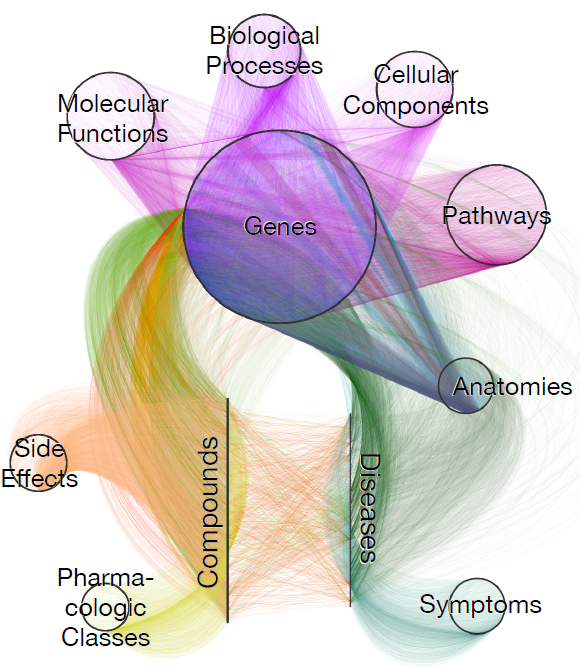
\includegraphics[width=0.8\columnwidth]{hetionet_graph.PNG}
    \caption[dummy]{
    Visualization of the heterogeneous biomedical network Hetionet\footnotemark.
    }
    \label{fig:biomedical_network}
\end{figure}
\footnotetext{\copyright\;Himmelstein et al.~\yrcite{himmelstein2017systematic}, licensed under \href{https://creativecommons.org/licenses/by/4.0/}{CC BY 4.0}.}
From a machine learning perspective, reasoning on biomedical KGs presents new challenges for existing approaches because of the unique structural characteristics of the graphs. One challenge arises due to the highly coupled nature of entities in biological systems that leads to many high-degree and densely interlinked entities.
A second challenge is the requirement of information beyond second-order neighborhoods for reasoning about the relationship between two entities~\cite{himmelstein2017systematic} so that 
%The combination of the requirement to consider multi-hop neighborhoods together with high-degree entities is difficult because
approaches where long-range interactions are incorporated only via node embeddings (e.\,g., RESCAL~\cite{nickel2011three}, TransE~\cite{bordes2013translating}) tend to underperform. %\textsc{comment: I would argue that the latent representations lead to long range interactions, also in RESCAL, as Nickel has shown?} 
Unfortunately, approaches that explicitly take the entire multi-hop neighborhoods into account (e.\,g., graph convolutional models, R-GCN~\cite{schlichtkrull2018modeling}), often have diminishing performance beyond two-hop neighborhoods (i.\,e., more than two convolutional layers). Furthermore,  high-degree entities can cause the aggregation operations to smooth out the signals. Alternatively, symbolic reasoning approaches (e.\,g., RuleN~\cite{meilicke2018fine}, AnyBURL~\cite{meilicke2019anytime}) learn logical rules and employ them during inference. However, due to the massive scale and diverse topologies of many real-world KGs, combinatorial complexity often prevents the usage of symbolic approaches. Also, logical inference has difficulties handling noise in the data. Recently, path-based reasoning methods have become popular, and they present a seemingly ideal balance for combining information over multi-hop neighborhoods. 
%The key challenge is finding meaningful paths, which can be computationally difficult if the search is not guided by domain principles. 

We propose a novel neuro-symbolic KG reasoning approach that combines path-based approaches with representation learning and logical rules.
These rules can be either mined from data or obtained from domain experts. Inspired by existing methods~\cite{minerva,lin2018multi,hildebr2020scene, hildebrandt2020reasoning}, we use reinforcement learning to train an agent to conduct policy-guided random walks on a KG. We propose a modification by introducing a reward function that allows the agent to leverage background knowledge formalized as metapaths. 
%Our results demonstrate that 
%existing methods for KG reasoning are inadequately designed to perform ideally in the unique structural characteristics of biomedical data. Furthermore, 
%we can overcome some of the weaknesses of existing methods. 
%by combining path-based reinforcement learning with symbolic knowledge in the form of logical rules.
In summary, our paper makes the following contributions:
\begin{itemize}
    \item We propose a novel neuro-symbolic approach that combines neural multi-hop reasoning based on reinforcement learning with logical rules.
    \item We conduct an empirical study of several state-of-the-art algorithms applied to a large biomedical KG.
    \item We show that our proposed approach outperforms state-of-the-art alternatives on a highly relevant biomedical prediction task (drug repurposing).
    %with respect to the standard metrics hits@$k$ for $k \in \{1,3,10\}$ and the mean reciprocal rank.
    %\item We show that explainable models are capable of scaling to large data sets and can even outperform black-box models on a real-world prediction task.
\end{itemize}
\noindent
%In support of reproducible research, we will provide supplementary material containing all necessary data and implementations for our experiments.

%The remainder of this work is organized as follows. We briefly introduce the notation and review the related literature in Section \ref{sec:background}. In Section \ref{sec:our_method}, we propose our method. Section \ref{sec:experiments} details an experimental study. 
%Furthermore, through ablative studies, we show how ... contribute to the results and examine the reasoning capabilities of MODELNAME in a controlled setting. 
%We  conclude in Section \ref{sec:conclusion}.



%[Comment: Wenn man es genau nimmt interagieren (korrelieren) nicht Entitäten, sondern triples die die  Entitäten beinhalten; Also nicht Gene1 mit Gene2, sondern der Expressiongrad von G1 mit dem von G2 ... Man kann natürlich das Prädikat "interagiert mit" einführen ... dann stimmt es vermutlich wieder  ]

%We then propose an novel approach by coupling symbolic knowledge with a reinforcement learning method to strike a balance that leads to superior performance for a reasoning task on a biomedical knowledge graph. Surprisingly, we are able to achieve superior performance while also maintaining 

%Machine learning methods in KGs have matured recently, but still suffer from their black-box nature and the need for large amounts of labeled examples. Decision making in biomedical domains is highly sensitive, therefore the importance of incorporating prior knowledge, e.g. in form of logical rules, during training and inference is essential for the adoption of ML. 

%Reasoning on biomedical KGs pose a unique challenge to ML approaches because of long-range path dependencies and very sparse links of interest (e.g. compound treats disease links).
% Can we include a Figure with a sub-graph from e.g. Neo4J?
%%%%%%%%%%%%%%%%%%%%%%%%%%%%%%%%%%%%%%%%%%%%%%%%%%%%

%Classical KG reasoning approaches are concerned with constructing explicit, symbolic rules (EXAMPLES; ILP? FOIL?) which can be used for inference by matching the body of the rule with instance data... However, due to the massive scale and diverse topologies of many real-world KGs, combinatorial complexity often prevents the usage of symbolic approaches. Even though recent rule-based techniques achieve state-of-the-art performance (e.g., \cite{meilicke2018fine} or \cite{meilicke2020reinforced}), most methods that are currently used follow the sub-symbolic representation learning paradigm. Instead of employing algorithms that directly operate on the input KG, the idea is to embed graph structures into low-dimensional vector spaces. New knowledge can be derived by exploiting statistical connectivity patterns via trainable functionals that operate on the embedding space. However, these methods suffer from the black-box problem and limited inference capabilities in situations where reasoning over complex paths is required. 




% We study its performance   in comparison with alternative state-of-the art reasoning methods and how they might be able to overcome weaknesses present in current approaches. We propose a novel neuro-symbolic KG reasoning approach that combines representation learning and logical rules.


As an application of our method, we focus on the drug repurposing problem, which is characterized by finding new treatment targets for existing drugs. By repurposing existing drugs, available knowledge about drug-disease-interactions can be leveraged to reduce time and cost for developing new drugs significantly. A recent example is the repositioning of the medication remdesivir for the novel coronavirus disease COVID\nobreakdash-19. 
%Remdesivir is a medication originally developed for hepatitis C, which was then repurposed for treating Ebola. Because of the antiviral properties of Remdesivir, first clinical trials are investigating the efficacy of this drug for a treatment of COVID-19. 
We aim at generating candidates for the drug repurposing task with machine learning reasoning methods and  formulate the task as a link prediction problem, where both compounds and diseases correspond to entities in a KG. 
%Interpretability and explainability of results are particularly important in the biomedical domain, and we use explicit logical rules in our method as background knowledge to obtain more transparent explanations.     

\section{Notation}
\label{sec:background}
\begin{figure}
    \centering
    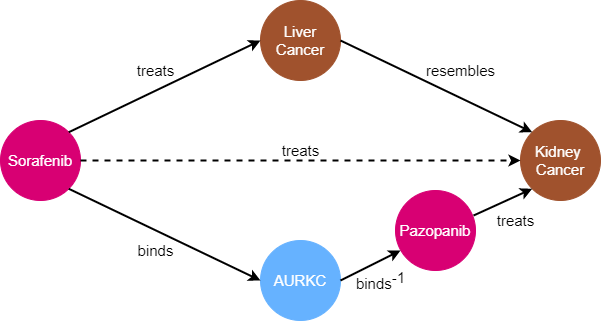
\includegraphics[width=0.9\columnwidth]{kg_example_sorafenib.png}
    \caption{Subgraph of Hetionet that illustrates the drug repurposing use case: The two paths that connect the chemical compound sorafenib and the disease kidney cancer can be used to predict a direct edge between the two entities.}
    \label{fig:kg_example}
\end{figure}
Let $\mathcal{E}$ denote the set of entities in a KG and $\mathcal{R}$ the set of binary relations. Elements in $\mathcal{E}$ correspond to biomedical entities including, e.\,g., chemical compounds, diseases, and genes. Each entity belongs to a unique type in $\mathcal{T}$, defined by the mapping $\tau : \mathcal{E} \rightarrow \mathcal{T}$. For example,  $\tau(\textit{AURKC}) =~\textit{Gene}$ indicates that the entity \textit{AURKC} has type \textit{Gene}. 
%Relations specify how  entities are connected. 
We define a KG $\mathcal{KG} \subset \mathcal{E} \times \mathcal{R} \times \mathcal{E} $ as a collection of triples of the form $(h, r, t)$, which consists of head, relation, and tail. 
%From a graphical point of view, 
Head and tail entities correspond to nodes in the graph, while the relation indicates the type of edge between them. For any relation $r \in \mathcal{R}$, we denote the corresponding inverse relation with $r^{-1}$  (i.\,e., $(h, r, t)$ is equivalent to $(t, r^{-1}, h)$). Triples in $\mathcal{KG}$ are interpreted as true known facts. For example, the triple 
%\textsc{(COMMENT: the standard is LiverCancer (one word), ...)}
$(\textit{Sorafenib}, \textit{treats}, \textit{Liver Cancer}) \in \mathcal{KG}$ 
in Figure \ref{fig:kg_example} corresponds to the fact that the kinase inhibitor drug sorafenib is approved for the treatment of liver cancer. 
%The \textit{treats} relation is of particular importance for this work since we frame the task of drug repurposing as a link prediction problem with respect to edges of type \textit{treats}.  The domain of \textit{treats} consists of chemical compounds, and the range is given by the set of all diseases. 

We further distinguish between two types of paths: instance paths and metapaths.
An instance path of length $T \in \mathbb{N}$ on $\mathcal{KG}$ is given by a sequence  
$$(e_1 \xrightarrow{r_1} e_2 \xrightarrow{r_2} \cdots \xrightarrow{r_{T}} e_{T+1}),$$ 
where $(e_i, r_i, e_{i+1}) \in \mathcal{KG}$. Moreover, we call 
$$(\tau(e_1) \xrightarrow{r_1} \tau(e_2) \xrightarrow{r_2} \cdots \xrightarrow{r_{T}} \tau(e_{T+1}))$$ a metapath. 
For example,
$$(\textit{Sorafenib} \xrightarrow{\textit{treats}} \textit{Liver Cancer} \xrightarrow{\textit{resembles}} \textit{Kidney Cancer})$$ constitutes an instance path of length 2, where $$(\textit{Compound} \xrightarrow{\textit{treats}} \textit{Disease} \xrightarrow{\textit{resembles}} \textit{Disease})$$ is the corresponding metapath. 
%[Comment: it is probably not necessary, but should we add the $\forall$ and the $\exists$ to the rules ....]


Logical rules (e.g., the commonly used Horn clauses) 
%that are typically employed for KG reasoning 
are usually written in the form $\textit{head} \leftarrow \textit{body}$. 
%In this work, we only consider rules where the head of a rule (not to be confused with the head entity in a triple) is a binary atom with respect to the \textit{treats}-relation. 
The head can be written out as a triple, and the body can be expressed as a metapath. Define $\textit{CtD} :=~(\textit{Compound}, \textit{treats}, \textit{Disease})$.
Then, a rule with respect to edges of type \textit{treats} is of the generic form
$$ \textit{CtD}  \leftarrow \left(\textit{Compound} \xrightarrow{r_1} \textit{Type}_2 \xrightarrow{r_2} \dots \xrightarrow{r_T} \textit{Disease} \right).
$$
In particular, the body of a rule corresponds to a metapath starting at a compound and terminating at a disease. The goal is to find instance paths where the corresponding metapaths match the body of a rule to predict a new relation between the source and the target of the instance path. The confidence of a rule indicates how often a rule is correct and is defined as the rule support divided by the body support in the data. 

\if false
For example, consider the rule
\begin{align*}
\textit{CtD} &\leftarrow \\ &(\textit{Compound} \xrightarrow{\textit{binds}} \textit{Gene} \xrightarrow{\textit{binds}^{-1}} \\& \textit{Compound} \xrightarrow{\textit{treats}} \textit{Disease}).
\end{align*}
The metapath of the following instance path
\begin{align*}
&(\textit{Sorafenib} \xrightarrow{\textit{binds}} \textit{AURKC} \xrightarrow{\textit{binds}^{-1}} \textit{Pazopanib} \\ &\xrightarrow{\textit{treats}} \textit{kidney cancer})
\end{align*}
matches the rule body, suggesting that sorafenib can also treat kidney cancer. %An explanation for this prediction can be elicited from the path by seeing that Zolmitriptan is similar to Rizatriptan, which is known to treat migraine.
\fi

\if false
\subsection{Related Work}
Even though real-world KGs contain a massive number of triples, they are still expected to suffer from incompleteness in the sense that true facts are missing. Therefore, link prediction (also known as KG completion) is a common reasoning task on KGs. Moreover, many classical artificial intelligence tasks such as  recommendation problems or question answering can be rephrased in terms of link prediction in KGs. In this work, we frame the drug repurposing task as a link prediction problem on a biomedical KG. 

Symbolic approaches have a far-reaching tradition in the context of knowledge acquisition and reasoning. The task of reasoning with logical rules has been addressed in areas such as Markov logic networks \cite{richardson2006markov} or inductive logic programming \cite{muggleton1991inductive}. However, such techniques typically do not scale well to modern, large-scale KGs. Recently, novel methods such as RuleN \cite{meilicke2018fine} and its successor AnyBURL \cite{meilicke2019anytime} have been proposed that achieve state-of-the-art performance on popular benchmark datasets such as FB15k-237 \cite{toutanova2015representing} and WN18RR \cite{dettmers2018convolutional}. %However, we find in our experiments (see Section \ref{sec:experiments}) that AnyBURL struggles to find rules on the biomedical KG that we consider in this paper.

Subsymbolic approaches map symbolic entities such as nodes and edges in KGs to low-dimensional vector representations known as embeddings. Then, the likelihood of missing triples is approximated by a classifier that operates on the embedding space. Popular embedding-based link prediction methods include translational methods such as TransE \cite{bordes2013translating} and TransR \cite{lin2015learning} or the tensor factorization approaches RESCAL \cite{nickel2011three} and ComplEx \cite{trouillon2016complex}. Moreover, R-GCNs~\cite{schlichtkrull2018modeling} were proposed, which extend graph convolutional networks \cite{kipf2016semi} to multi-relational graphs.

Despite achieving good results on the link prediction task, a fundamental problem of many embedding-based methods is their non-transparent nature in the sense that it remains hidden to the user what contributed to the  predictions. Moreover, most embedding-based methods cannot capture the compositionality expressed by long reasoning chains. This often limits their applicability to complex reasoning tasks. Multi-hop reasoning methods (also known as path-based methods) follow a different philosophy than embedding-based methods. The underlying idea is to infer missing knowledge based on extracting paths from the KG. Thereby, these methods come with an inherent transparency mechanism by providing explicit reasoning chains that can be analyzed by the user. The pioneering method Path Ranking Algorithm (PRA) \cite{lao2010relational} formulates the link prediction task as a maximum likelihood classification based on paths sampled from a nearest neighbor random walk. Xiong et al.\;extend the idea from PRA and frame the task of path extraction as a reinforcement learning problem~\cite{wenhan_emnlp2017}. They propose DeepPath, which substitutes the nearest neighbor random walk from PRA with a policy-guided random walk. The method that we propose in this work is an extension of the path-based method MINERVA \cite{minerva}. The underlying mechanism is to train a reinforcement learning agent to perform a policy-guided random walk until the answer entity to a query is reached. The goal is that the agent's policy implicitly encodes fuzzy logical rules that generalize to unseen test instances.

One of the drawbacks of existing policy-guided walk methods is that the agent might receive noisy reward signals based on corrupted or spurious triples that lead to the correct answer entity during training, but lower the generalization capabilities during testing. Moreover, biomedical KGs often exhibit both long-range dependency structures and high-degree hub nodes (see Section~\ref{sec:dataset}). %(often given by entities of type $gene$). 
The combination of these two properties makes it difficult for MINERVA's agent to navigate over biomedical KGs and extend a path in the most promising way. As a remedy, we propose the incorporation of known, effective logical rules via a novel reward function. This can help to denoise the reward signal and guide the agent on long paths with high-degree nodes.

%neuro-symbolic \cite{lamb2020graph}

\fi

\section{Our Method}
\label{sec:our_method}

We pose the task of drug repurposing as a link prediction problem based on graph traversal. Starting at a query entity (e.g., a compound to be repurposed), an agent performs a walk on the graph by sequentially transitioning to a neighboring node. The decision of which transition to make is determined by a stochastic policy. Each subsequent transition is added to the current path, extending the reasoning chain, until a finite number of transitions is reached. 
%The stochastic walk process iterates until a finite number of transitions (defined by a hyperparameter) has been made. 
The general approach is inspired by the reinforcement learning method MINERVA~\cite{minerva}, with our primary contribution coming from the incorporation of logical rules into the training process.% More formally, the agent's learning task is modeled via the fixed-horizon Markov decision problem outlined below.

\sloppy 
The state of the environment consists of the entity $e_t$ where the agent is located at time $t$, the source entity $e_c$, and the target entity $e_d$, where $e_c$ and $e_d$ correspond to the compound that we aim to repurpose and the target disease, respectively. %\textsc{Seems to be an unusual definition of a state}
Thus, a state $S_t$ for time $t \in \mathbb{N}$ is represented by $S_t := \left(e_t, e_c, e_d\right)$. The agent is given no information about the target disease so that the observed part of the state space is given by $\left(e_t, e_c\right) \in \mathcal{E}^2$.
Let $\boldsymbol{e} \in \mathbb{R}^{d}$ denote the embedding of entity $e$ and $\boldsymbol{r} \in \mathbb{R}^{d}$ the embedding of relation $r$.
The set of available actions contains all outgoing edges from the node $e_t$ with the corresponding target nodes and the option to stay at the current node with no transition. We denote with $A_t \in \mathcal{A}_{S_t}$ the action that the agent performed at time $t$. The environment evolves deterministically by updating the state according to the previous action. 

 The agent encodes previous actions via a multi-layered LSTM \cite{hochreiter1997long}
\begin{equation}
\label{eq:lstm_agent}
        \boldsymbol{h}_t = \text{LSTM}\left(\left[\boldsymbol{a}_{t-1}, \boldsymbol{e}_c\right]\right),
\end{equation}
where $\boldsymbol{a}_{t-1} := \left[\boldsymbol{r}_{t-1},\boldsymbol{e}_{t}\right] \in \mathbb{R}^{2d}$ corresponds to the vector space embedding of the previous action (or the zero vector at time $t=0$).
%, with $\boldsymbol{r}_{t-1}$ and $\boldsymbol{e}_{t}$ denoting the embeddings of the relation and the target entity in $\mathbb{R}^{d}$, respectively. Moreover, $\boldsymbol{e_c} \in \mathbb{R}^{d}$ encodes the source compound. 
The action distribution is given by
\begin{equation}
\label{eq:policy_agent}
\boldsymbol{d}_t = \text{softmax}\left(\boldsymbol{A}_t \left(\boldsymbol{W}_2\text{ReLU}\left(\boldsymbol{W}_1 \boldsymbol{h}_t\right)\right)\right),
\end{equation}
where $\boldsymbol{W_1}$ and $\boldsymbol{W_2}$ are weight matrices and the rows of $\boldsymbol{A}_t \in \mathbb{R}^{\vert \mathcal{A}_{S_t} \vert \times 2d}$ contain the latent representations of all admissible actions from $S_t$. An action $A_t \in \mathcal{A}_{S_t}$ is sampled according to
$
    A_t \sim \text{Categorical}\left(\boldsymbol{d}_t\right).
$
Overall, $T$ transitions are sampled, resulting in a path denoted by $$
    P := (e_c \xrightarrow{r_1} e_2 \xrightarrow{r_2} \dots \xrightarrow{r_{T}} e_{T+1}) ,
$$ 
where $T$ is the maximum path length. 
Equations \eqref{eq:lstm_agent} and \eqref{eq:policy_agent} induce a stochastic policy, represented by $\pi_{\boldsymbol{\theta}}$ where $\boldsymbol{\theta}$ denotes the set of all trainable parameters, including all entity and relation embeddings.

Furthermore, let $\mathcal{M}~=~\{M_1, M_2, \dots, M_m\}$ be the set of metapaths, where each element corresponds to the body of a rule. %[conjunct (or whatever the right term is) of a rule body] 
For every metapath $M$, we assign a score $S(M)\in \mathbb{R}$ that indicates a quality measure of the corresponding rule, such as the confidence or the support with respect to making a correct prediction. For a path $P$, we denote with $\Tilde{P}$ the corresponding metapath. 

During training, a terminal reward is computed according to
\begin{equation*}
\label{eq:rewards}
    R =  \mathbb{I}_{\{e_{T+1} = e_d\}}\left(1 + \lambda \sum_{i = 1}^m S(M_i) \mathbb{I}_{\{\Tilde{P} = M_i\}}\right).
\end{equation*}
The first term indicates whether the agent has reached the correct target disease. The second term checks whether the metapath corresponds to the body of a rule and adds to the score accordingly. Heuristically speaking, we want to reward the agent with a higher score for extracting a metapath that corresponds to a body. The hyperparameter $\lambda \geq 0$ balances the two components of the reward. For $\lambda = 0$, we recover MINERVA.

We employ REINFORCE \cite{williams1992simple} to maximize the expected rewards. Thus, the agent's maximization problem is given by
\begin{equation}
\label{eq:objective_agent}
    \argmax_{\boldsymbol{\theta}} \mathbb{E}_{e_c \sim \mathcal{E}_c}\mathbb{E}_{A_1, A_2, \dots, A_{T} \sim \pi_{\boldsymbol{\theta}}}\left[R \mid e_c \right]  ,
\end{equation}
where $\mathcal{E}_c$ denotes the true underlying distribution of the set of chemical compounds.
%During training, the first expectation in Equation \eqref{eq:objective_agent} is substituted with the empirical average over the training set. The second expectation is approximated by the empirical average over multiple rollouts. %We also employ a moving average baseline to reduce the variance. Further, we use entropy regularization with parameter $\beta\in \mathbb{R}_{\geq 0}$ to enforce exploration.% \textsc{So in testing, the agent is not informed about the disease, since we are looking for repurposing.  So it could end up at any disease! Can you make this clearer}

\section{Experiments}
\label{sec:experiments}
\subsection{Dataset}
\label{sec:dataset}
Hetionet ~\cite{himmelstein2017systematic} is a biomedical KG that integrates data from 29 highly reputable and cited public databases.
%, including the Unified Medical Language System (UMLS) \cite{bodenreider2004unified}, Gene Ontology \cite{ashburner2000gene}, and DrugBank \cite{wishart2006drugbank}.
It consists of 47,031 entities with 11 different types and 2,250,197 edges with 24 different types. 
We aim to predict edges with type \textit{treats} between entities that correspond to compounds and diseases. The goal is to perform candidate ranking according to the likelihood of successful drug repurposing in a novel treatment application.  
There are 1552 compounds and 137 diseases in Hetionet with 775 observed links of type \textit{treats} between compounds and diseases. 

\if false
Figure~\ref{fig:metagraph} illustrates the schema and shows the different types of entities and possible relations between them.

\begin{figure}[t!]
    \centering
    \includegraphics[width=0.75\textwidth]{figures/metagraph.png}
    \caption{Metagraph of Hetionet \cite{himmelstein2017systematic}\textsuperscript{1}: Hetionet has 11 different entity types and 24 possible relations between them.}
    \label{fig:metagraph}
    \vspace{2mm}
\end{figure}

Hetionet differs in many aspects from the standard benchmark datasets that are typically used in the KG reasoning literature. Table \ref{tab:datasets} summarizes the basic statistics of Hetionet along with the popular benchmark dataset FB15k-237 \cite{toutanova2015representing} and WN18RR \cite{dettmers2018convolutional}. One of the major differences between Hetionet and the two other benchmark datasets is the density of  triples with respect to the number of entities. It means that the average node degree in Hetionet is significantly higher than in the other two KGs. In addition, Figure  \ref{subfig:degrees} illustrates the average degrees for the different entity types in Hetionet. It is apparent that entities of type \textit{Anatomy} are densely connected hub nodes. In addition, entities of type \textit{Gene} have an average degree of around 123. This plays a crucial role for our application since many relevant paths that connect \textit{Compound} and \textit{Disease} traverse entities of type \textit{Gene} (see Figure \ref{fig:metagraph} and Table \ref{tab:metapaths}). We will discuss in Section~\ref{subsec:discussion} further how particularities of Hetionet impose challenges for existing KG reasoning methods.
%\textsc{Comment: maybe in the table you can remind the reader that these describe the rule bodies and the rule head is always (Compound, treats,  Disease)}


\begin{table}[t!]
\caption{Comparison of Hetionet with the two benchmark datasets FB15k-237 and WN18RR.}
\center
\resizebox{\columnwidth}{!}{
\begin{tabular}{ c  c  c  c c}
 \hline
 Dataset & Entities & Relations & Triples & Avg. degree \\
 \hline \hline
Hetionet & 47,031 & 24 & 2,250,197 & 95.8\\
FB15k-237 & 14,541 & 237 & 310,116 & 19.7\\
WN18RR & 40,943 & 11 & 93,003 & 2.2 \\
%NELL-995 & 75,492 & 200 & 154,213
 \vspace{0.2cm}
\end{tabular}
}
\label{tab:datasets}
\end{table}
\if false
\begin{figure}[t]
    \begin{subfigure}{0.45\textwidth}
        \includegraphics[width=\linewidth]{figures/entity_counts.png} 
        \caption{Entity counts}
        \label{subfig:counts}
    \end{subfigure}
    \begin{subfigure}{0.45\textwidth}
        \includegraphics[width=\linewidth,center]{figures/entity_degree.png}
        \caption{Average node degrees}
        \label{subfig:degrees}
    \end{subfigure}
    \caption{Comparison of the total counts (a) and the average node degrees (b) according to each entity type in Hetionet.}
    \label{fig:counts_degrees}
\end{figure}
\fi
\fi

%We randomly split these 755 triples into training, validation, and test set, where the training set contains 483 triples, the validation set $121$ triples, and the test set 151 triples.% The data split will be made public along with the code in the final version of this paper.

\subsection{Metapaths as Background Information}

Himmelstein et al.~\yrcite{himmelstein2017systematic} compiled a list of 1206 metapaths corresponding to various pharmacological efficacy mechanisms that connect entities of type \textit{Compound} with entities of type \textit{Disease}. Through hypothesis testing and domain expertise, they identified $31$ effective metapaths that served as features for a logistic regression model. %that outputs a treatment probability of a compound for a disease. 
Out of these metapaths, we select the 10 metapaths as background information that have at most path length 3 and exhibit positive regression coefficients, indicating their importance for predicting drug efficacy. The metapaths are included as rule bodies in $\mathcal{M}$, where the rule head is always \mbox{(\textit{Compound}, \textit{treats}, \textit{Disease})}. We estimate the confidence score for each rule by sampling 10,000 paths whose metapaths correspond to the rule body and use the confidence for the score $S(M)$  (see Section {\ref{sec:our_method}}).
Table \ref{tab:metapaths} shows the three metapaths with the highest confidences.

\begin{table}
\caption{Three metapaths and their scores.}
\begin{center}
\resizebox{0.95\columnwidth}{!}{
\begin{tabular}{c|l}
$S(M)$ & Metapath $M$\\
\hline
\hline
0.446 & $(\textit{Compound} \xrightarrow{\textit{includes}^{-1}} \textit{Pharmacologic Class} \xrightarrow{\textit{includes}} \textit{Compound}$\\
& $\hspace{1mm} \xrightarrow{\textit{treats}} \textit{Disease})$\\
0.265 & $(\textit{Compound} \xrightarrow{\textit{resembles}} \textit{Compound} \xrightarrow{\textit{resembles}} \textit{Compound} \xrightarrow{\textit{treats}} \textit{Disease})$ \\
0.184 & $(\textit{Compound} \xrightarrow{\textit{binds}} \textit{Gene} \xrightarrow{\textit{associates}^{-1}} \textit{Disease})$
\end{tabular}
}
\label{tab:metapaths}
\end{center}
\end{table}

\if false
0.182 & $(\textit{Compound} \xrightarrow{\textit{resembles}} \textit{Compound} \xrightarrow{\textit{treats}} \textit{Disease})$\\
0.169 & $(\textit{Compound} \xrightarrow{\textit{palliates}} \textit{Disease} \xrightarrow{\textit{palliates}^{-1}} \textit{Compound} \xrightarrow{\textit{treats}} \textit{Disease})$\\
0.143 & $(\textit{Compound} \xrightarrow{\textit{binds}} \textit{Gene} \xrightarrow{\textit{binds}^{-1}} \textit{Compound} \xrightarrow{\textit{treats}} \textit{Disease})$\\
0.058 & $(\textit{Compound} \xrightarrow{\textit{causes}} \textit{Side Effect} \xrightarrow{\textit{causes}^{-1}} \textit{Compound} \xrightarrow{\textit{treats}} \textit{Disease})$\\
0.040 & $(\textit{Compound} \xrightarrow{\textit{treats}} \textit{Disease} \xrightarrow{\textit{resembles}} \textit{Disease})$\\
0.017 & $(\textit{Compound} \xrightarrow{\textit{resembles}} \textit{Compound} \xrightarrow{\textit{binds}} \textit{Gene} \xrightarrow{\textit{associates}^{-1}} \textit{Disease})$ \\
0.004 & $(\textit{Compound} \xrightarrow{\textit{binds}} \textit{Gene} \xrightarrow{\textit{expresses}^{-1}} \textit{Anatomy} \xrightarrow{\textit{localizes}^{-1}} \textit{Disease})$ \\
\fi

\subsection{Experimental Setup}
We apply our method, denoted by MINERVA+, to Hetionet and calculate hits@1, hits@3, hits@10, and the mean reciprocal rank (MRR).
During inference, a beam search is carried out, and the entities are ranked by the probability of their corresponding paths. 
Moreover, we consider another evaluation scheme (MINERVA+ (pruned)) that retrieves and ranks only those paths from the test rollouts that correspond to one of the metapaths.
%in Table \ref{tab:metapaths}. 
All the other extracted paths are not considered in the ranking. 
We compare our approach with the path-based method MINERVA, the rule-based method AnyBURL, and the embedding-based methods TransE, RESCAL, and R-GCN.

\if false
For our method, the hyperparameter $\lambda$ that balances the two rewards (see Equation \ref{eq:rewards}) is chosen from the range $\{1,2,3,4,5\}$. The embedding size is tuned from $\{32, 50, 128\}$, and the hidden size of the MLP-layers for the action distribution is selected from $\{32, 50, 128, 256\}$. The number of LSTM-layers in the policy of the agent is chosen from $\{1, 2\}$, and the entropy regularizer $\beta$ takes values in $\{0.02, 0.05\}$. The path length is set to 3, the number of rollouts is given by 40 for training, and the beam width (number of test rollouts) at inference time is set to 100.

We compare our results with the following baseline methods. AnyBURL \cite{meilicke2019anytime} is a rule-based method that first mines logical rules by sampling paths in the graph and estimating the confidence of the rules. Then, it predicts candidates for link prediction, which are generated by applying the learned rules. %We use the default parameters and learn the rules for $1000$ seconds. %AnyBURL reports the filtered metrics, which act as an upper bound of the unfiltered metrics. 
We test AnyBURL also in an additional setting (AnyBURL (metapaths)): Instead of applying the learned rules for prediction, we use the rules derived from the metapaths in Table \ref{tab:metapaths} for inference.
% The MRR is a lower bound since AnyBURL only calculates the first $k$ possible objects...

The methods TransE \cite{bordes2013translating} and RESCAL \cite{nickel2011three} are both embedding-based models. TransE defines additive functions over the embeddings and employs distance-based scoring. RESCAL aims to compute a low-rank approximation of the adjacency tensor corresponding to a KG.
%For both methods, we choose the embedding dimension from the set $\{32, 64, 128, 256\}$ and the margin $\gamma$ for the loss from $\{0.1, 1, 2\}$. For negative sampling, we choose $10$ negative subjects and either $10$ or $50$ negative objects for each triple. 
To cover a more recent paradigm in graph-based machine learning, we include a baseline graph convolution approach to compute KG embeddings given by the relational graph convolutional network R-GCN \cite{schlichtkrull2018modeling}. Extending the idea from the graph convolutional network GCN \cite{kipf2016semi} to multi-relational graphs, R-GCN mimicks the convolution operator on regular grids where an entity embedding is formed by aggregating node features from its neighbors. %We use a two layer R-GCN model and the hyperparameters we explore are embedding dimensions $\{8, 16, 32\}$ and learning rates $\{0.1, 0.01, 0.001\}$.

%The exact hyperparameter settings for all models are provided in the supplementary material to ensure reproducibility of the results.

%All experiments were conducted on a machine with 16
%CPU cores and 32 GB RAM. Training our method on the Hetionet dataset takes around 10 minutes, testing about 10 seconds.

%\begin{table*}
%\begin{center}
%{\caption{Optimal hyperparameters.}
%\label{tab:hyperparameters}}
%\begin{tabular}{|c|c|}
%\hline
%Method & Hyperparameters\\
%\hline
%AnyBURL   & ...\\
%\hline
%TransE   & \\
%\hline
%RESCAL   & \\
%\hline
%MINERVA/+  & \\
%\hline
%\end{tabular}
%\end{center}
%\end{table*}
\fi

\subsection{Results}
\label{sec:results}

\begin{table}[h]
\caption{Comparison with baseline methods.% MINERVA+ outperforms the baseline methods in all evaluation metrics.
}
\begin{center}
\resizebox{0.95\columnwidth}{!}{
\begin{tabular}[H]{c c c c c}
Method & Hits@1 & Hits@3 & Hits@10 & MRR\\
\hline
\hline
AnyBURL & $0.139$ & $0.254$ & $0.358$ & $0.210$ \\
AnyBURL  (metapaths) & $0.252$ & $0.364$ & $0.609$ & $0.354$\\
TransE  & $0.073$ & $0.172$ & $0.318$ & $0.161$ \\
RESCAL  & $0.205$& $0.35$ &$0.576$ & $0.317$ \\
R-GCN  & $0.093$ &$0.245$ & $0.364$ & $0.188$ \\
MINERVA & $0.249$&$0.391$ & $0.605$& $0.357$\\
\hline
MINERVA+   & $0.294$& $0.437$&$0.615$ &$0.396$  \\
MINERVA+ (pruned)  & $\mathbf{0.319}$& $\mathbf{0.468}$&$\mathbf{0.628}$ &$\mathbf{0.416}$  \\
\end{tabular}
}
\label{tab:results}
\end{center}
\end{table}

Table \ref{tab:results} displays the test results for the experiments. 
%Due to the random sampling of the training rollouts, the training procedure of MINERVA and MINERVA+ are essentially random processes. 
The reported values for MINERVA and MINERVA+ correspond to the mean across five independent training runs. The standard errors lie between $0.0072$ and $0.0198$. This indicates that the reported performance gains are highly significant. %However, additional work is required to reduce the variance.


%AnyBURL finds ... rules for the relation $treats$ during training, of which only one rule corresponds to the metapaths in \ref{tab:metapaths. 
AnyBURL only learns one rule for the relation $treats$ that has a length of at least 2. 
%This rule corresponds to the fourth metapath in Table \ref{tab:metapaths}.
%which leads to a lowest performance among all considered methods. 
To see the effect of applying a larger number of rules, we try a setting where we use the metapaths for the prediction step, which leads to significantly improved results.
TransE and R-GCN show similar performance, and RESCAL performs best among the embedding-based methods.
%MINERVA+ outperforms all baseline methods with respect to all evaluation metrics. 
Applying the modified ranking scheme, our method yields performance gains of $26.6\%$ for hits@1, $19.7\%$ for hits@3, $3.1\%$ for hits@10, and $16.5\%$ for MRR with respect to best performing baseline method.% This confirms the validity of using logical rules for guiding the reinforcement learning agent.
%During training, all 10 metapaths are extracted by our method. 
 
%In order to evaluate whether our method incorporates the presented metapaths that lead to correct predictions, we monitor the number of extracted instance paths that match a metapath from Table \ref{tab:metapaths} during training. A comparison of the relative frequency of such instance paths across all 5 training runs between MINERVA and our method is shown in Figure \ref{fig:rule_count_train}. The proportion of these paths in MINERVA and our method is approximately the same for the first 60 iteration. However, in the following 20 iterations the percentage of metapaths that lead to the correct entity increases at a steeper slope for our method and is $46.6\%$ higher at the end of training than for MINERVA. 
%During the test rollouts, MINERVA+ extracts rules for $44.6\%$ of the paths, while MINERVA extracts rules for $40.1\%$ of the paths.
%MINERVA+ extracts rules for $44.6\%$ of the paths, where $17.2\%$ end at the correct entity. For comparison, MINERVA extracts rules for $40.1\%$ of the paths, of which $16.2\%$ end at the correct entity.

\if false
\begin{figure}[t!]
    \centering
    \includegraphics[width=0.6\textwidth]{figures/rule_count_train_mean.png}
    \caption{Relative frequency of instance paths that correspond to a rule and lead to the correct entity during training. %For each iteration, we perform 20 rollouts.
    }
    \label{fig:rule_count_train}
\end{figure}
\fi

\if false
The metapath that was most frequently extracted is 
\begin{align*}
    &(\textit{Compound} \xrightarrow{\textit{causes}} \textit{Side Effect} \xrightarrow{\textit{causes}^{-1}} \textit{Compound} \\ & \xrightarrow{\textit{treats}} \textit{Disease}) \;.
    \label{eq:CcSE_metapath}
\end{align*}
This rule was followed in $33.1\%$ of the paths during testing, of which $15.3\%$ ended at the correct entity. 
The second most extracted metapath is 
\begin{align*}
&(\textit{Compound} \xrightarrow{\textit{includes}^{-1}} \textit{Pharmacologic Class} \\ & \xrightarrow{\textit{includes}} \textit{Compound}\xrightarrow{\textit{treats}} \textit{Disease})
\end{align*}
with a confidence of $35.5\%$.
\fi

%We notice that MINERVA extracts metapath \eqref{eq:CcSE_metapath} in 45.8\% of the test rollouts. This is probably due to the fact that there are almost 140,000 edges between nodes of the types \textit{Compound} and \textit{Side Effect}. From nodes of type \textit{Side Effect}, it is only possible to return to \textit{Compound}, and since we want to predict diseases, the best next step to be taken leads across the edge \textit{treats}. However, this rule has a low confidence and often leads to wrong results. Our method learns to follow other rules with higher confidence more often so that the prediction performance improves.



 
\if false
\begin{itemize}
    \item Add R-GCN \& metapath2vec
    \item Training efficiency (show training curves Minerva and 
    MINERVA+)
    \item Ablation study
\end{itemize}
\fi
\subsection{Discussion}
\label{subsec:discussion}
%We have integrated logical rules via a new reward mechanism into the multi-hop reasoning method MINERVA. 
%The policy incorporates the set of rules that are presented to the agent during training. 
%The method that is presented in this work is not limited to MINERVA, but 
Our method can act as a generic mechanism to inject domain knowledge into reinforcement learning-based reasoning methods on KGs~\cite{lin2018multi,wenhan_emnlp2017}. While we employ rules that are extracted in a data-driven fashion, our method is agnostic towards the source of background information.
The additional reward for extracting a rule (see Equation~\eqref{eq:rewards}) can be considered as a regularization that enforces the agent to walk along metapaths that generalize to unseen instances. 
%From a different point of view, the policy of the agent balances two objectives: extracting metapaths and predicting the correct target disease. In particular, for MINERVA+ (pruned), we consider only extracted paths that correspond to the input rules. However, the resulting ranking of these rules is not based on global quality measures of the rules (e.\,g., confidence). Rather, the ranking is given by the policy of the agent (i.\,e., metapaths that are more likely to be extracted are ranked higher), which induces an adaptive reweighting of the extracted rules that takes the individual instance paths into account.

AnyBURL is strictly outperformed by both MINERVA and our method. Most likely, the large amount of high-degree nodes in Hetionet lead to the outcome that hardly any strong, predictive rules are extracted. %We also considered the setting where AnyBURL performs inference based on the same metapaths that we used for our method. This leads to a significantly better outcome and lifts the performance of AnyBURL on the same level as MINERVA. However, our method still strictly outperforms both MINERVA and AnyBURL by a quite large margin. 
Multi-hop reasoning methods contain a natural transparency mechanism by providing explicit inference  paths. 
%These paths allows domain experts to evaluate and monitor the predictions. 
%Typically, there is an inherent trade-off between explainability and performance when choosing the appropriate machine learning model. 
Surprisingly, our experimental findings show that path-based reasoning methods outperform existing black-box methods on the drug repurposing task without a trade-off between explainability and performance. 
%Concretely, we compared our methods against the embedding-based methods TransE and RESCAL. 
Both TransE and RESCAL are trained to minimize the reconstruction error in the immediate first-order neighborhood,
%discarding higher-order proximities. However, the analysis by Himmelstein et al.\;showed that most explanatory metapaths in the drug repurposing setting have length 2 or more~\cite{himmelstein2017systematic}.
%While MINERVA and our method can explicitly reason over multiple hops, 
and our results indicate that these methods 
%that fit low-order proximities
seem not to be suitable for the drug repurposing task.
%, and 
%it is plausible that 
%other reasoning tasks on biomedical KGs could result in similar outcomes. %We expect that this result generalizes to other task in the biomedical domain where long-term dependencies play an important role such as finding associations between genes and disease.
%Both methods also have to be trained on the whole graph, wheras our method can focus on the triples in the training set since the agent just needs to know the local subgraph for determine the next action.
%R-CGNs learn node embeddings by aggregating incoming messages from neighboring nodes and combing this information with its own embedding. 
%The receptive field of an R-GCN with $k$ layers corresponds to the $k$-hop neighborhood of the center node. Thus, 
R-GCN is in principle capable of modeling long-term dependencies due to the receptive field containing the entire set of nodes in the multi-hop neighborhood. However, the aggregation and combination step of R-GCN essentially acts as a low-pass filter on the incoming signals, and 
%this can be problematic 
in the presence of many high-degree nodes, 
%such as in Hetionet, where 
the center nodes may receive an uninformative signal that smooths over the neighborhood embeddings. 

To illustrate the applicability of our method, consider the compound sorafenib from Figure \ref{fig:kg_example}.
%, which is known for treating liver cancer, kidney cancer, and thyroid cancer. 
The three highest predictions of our model for new target diseases include hematologic cancer, breast cancer, and Barrett's esophagus. 
%This result seems to be sensible since Sorafenib is known to treat three other cancer types. 
The database ClinicalTrails.gov \cite{national2007clinicaltrails} 
%from the U.\,S.\;National Library of Medicine (NLM) 
lists 23 clinical studies for testing the effect of sorafenib on these three diseases, showing that the predictions are meaningful targets for further investigation.  

%Because the entities in Hetionet have high node degress (see Figure \ref{fig:counts_degrees}), the signal could be smoothed out. Similarly, messages from further away neighbors lose their informativeness. 
%Our method overcomes the weaknesses of the other models. It is capable of multi-hop reasoning without losing information and is scalable to large datasets. Explicit paths leading to the correct answer are extracted, which act as explanations for the existence of the link.

%After hyperparameter tuning, the optimal path length was found to be 3. Since almost all given rules have a length up to 3, the information of the rules could be leveraged during training. For longer paths, it was rare for the agent to follow a rule because the agent does not tend to stay at the same node. To improve the performance for increased path lengths, one could consider exploring longer metapaths. 

%We have also tried the setting where an additional reward is given when only the path follows a rule body, but the end entity is incorrect. This resulted in an increased use of rules, but since the rules often do not lead to the correct entity, the performance of the model dropped.


%The methods TransE and RESCAL both only take the first-order neighborhood into account. However, the compounds and diseases are usually connected by paths of length at least 2. Both methods also have to be trained on the whole graph, wheras our method can focus on the triples in the training set since the agent just needs to know the local subgraph for determine the next action. 
%R-CGN learns node embeddings by aggregating incoming messages from neighboring nodes. Because the entities in Hetionet have high node degress (see Figure \ref{fig:counts_degrees}), the signal could be smoothed out. Similarly, messages from further away neighbors lose their informativeness. 


\if false
\begin{itemize}
    \item rule-based approaches and complexity
    \item policy-guided random walk vs nearest neighbor random walks
    \item R-GCN smoothes out important signals
    \item pretrained embeddings
    \item how important is the quality (confidence?) and quantity of the rules ablation study with a subset of the metapaths
    \item can we map our predictions to an existing medical study?
\end{itemize}
\fi

\section{Conclusion}
\label{sec:conclusion}
% Biomedical knowledge graphs impose challenges for learning algorithms that are not reflected in common benchmark datasets. 
%Our experimental findings suggest that existing knowledge graph reasoning methods face difficulties on Hetionet, a biomedical knowledge graph that exhibits both long-range dependencies and a multitude of high-degree nodes. 
We have proposed a novel neuro-symbolic knowledge graph reasoning approach that leverages path-based reasoning,  representation learning, and logical rules. 
We apply our method to the highly relevant task of drug repurposing and compare our approach with both embedding-based and rule-based methods. We achieve better performance and an improvement of $26.6\%$ for hits@1 and $16.5\%$ for the mean reciprocal rank compared to popular baselines. 
%Concretely, we integrate logical rules into a multi-hop reasoning method based on reinforcement learning via a novel reward mechanism. %The idea is to use the rules as background information to guide the walk of the reinforcement learning agent. 
%We apply our method to the highly relevant task of drug repurposing and compare our method with both embedding-based and rule-based methods. We achieve better performance and an improvement of $26.6\%$ for hits@1 and $16.5\%$ for the mean reciprocal rank compared to popular baseline methods. %Further, we empirically conform that the proposed reward mechanism leads to more rules being extracted during training and testing.   

\newpage
\section*{Acknowledgements}
This work has been supported by the German Federal Ministry for Economic Affairs and Energy (BMWi) as part of the project RAKI (no.\;01MD19012C).

\begin{figure}[h]
\centering
    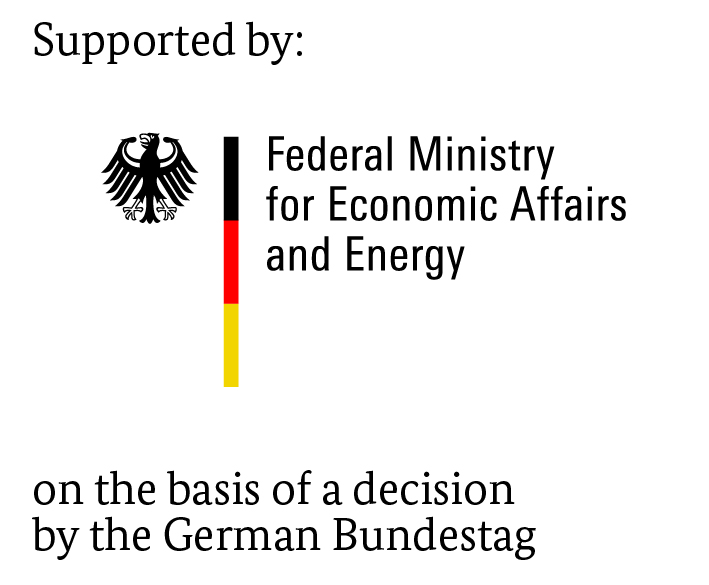
\includegraphics[width=0.5\columnwidth]{BMWi_4C_Gef_en.jpg}
\end{figure}


\bibliography{bibliography}
\bibliographystyle{icml2020}

\end{document}


% This document was modified from the file originally made available by
% Pat Langley and Andrea Danyluk for ICML-2K. This version was created
% by Iain Murray in 2018, and modified by Alexandre Bouchard in
% 2019 and 2020. Previous contributors include Dan Roy, Lise Getoor and Tobias
% Scheffer, which was slightly modified from the 2010 version by
% Thorsten Joachims & Johannes Fuernkranz, slightly modified from the
% 2009 version by Kiri Wagstaff and Sam Roweis's 2008 version, which is
% slightly modified from Prasad Tadepalli's 2007 version which is a
% lightly changed version of the previous year's version by Andrew
% Moore, which was in turn edited from those of Kristian Kersting and
% Codrina Lauth. Alex Smola contributed to the algorithmic style files.
